\section{Software}
\begin{frame}{Software}
	Our project is \stress{openly} and \stress{actively} developed on
	\vcenteredinclude{\includegraphics[height=2ex]{figures/software_logos/octocat.pdf}\hspace{-0.05cm}
	
\includegraphics[height=2ex]{figures/software_logos/github.pdf}}\\
	{\color{purple}\url{https://github.com/RD-clustering/B_decays_clustering}}
	
	\bigskip
	Implemented in \vcenteredinclude{\includegraphics[height=3ex]{figures/software_logos/python.pdf}} using
	\begin{itemize}
		\item \vcenteredinclude{\includegraphics[height=4ex]{figures/software_logos/numpy_noname.pdf}} \texttt{numpy} {\footnotesize(fast numeric operations on arrays)}
		\item \vcenteredinclude{
\includegraphics[height=3.5ex]{figures/software_logos/pandas_noname.pdf}} \texttt{pandas} {\footnotesize(dataframes)}
		\item \vcenteredinclude{\includegraphics[height=4ex]{figures/software_logos/matplotlib.pdf}} \texttt{matplotlib} {\footnotesize(beautiful plots)}
		\item \vcenteredinclude{\includegraphics[height=3.5ex]{figures/software_logos/sklearn.pdf}} \texttt{scikit-learn} {\footnotesize(clustering tools)}
		\item \vcenteredinclude{\includegraphics[height=3.5ex]{figures/software_logos/scipy.pdf}} \texttt{scipy} {\footnotesize(integration and clustering tools)}
		\item \vcenteredinclude{\includegraphics[height=3.5ex]{figures/software_logos/jupyter.pdf}} \texttt{jupyter} {\footnotesize(interactive notebooks)}
		\item \vcenteredinclude{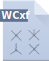
\includegraphics[height=3ex]{figures/software_logos/wcxf.pdf}} \texttt{wcxf} {\footnotesize(specify Wilson coefficients in a variety of bases)}
		\item \vcenteredinclude{\includegraphics[height=3ex]{figures/software_logos/wilson.pdf}} \texttt{Wilson} {\footnotesize(running of Wilson coefficients)}
		\item \vcenteredinclude{\includegraphics[height=3ex]{figures/software_logos/flavio.pdf}} \texttt{Flavio} {\footnotesize(various observables with NP predictions)}
	\end{itemize}
\end{frame}